\documentclass[plainreport]{cgvpub}
% other document types next to bachelorofscience:
% masterofscience
% diplominf
% diplomist
% beleg

%more options (to be appended in the square brackets):
% german....... german version 
% female........ to be used for female endings in german
% bibnum....... numerical reference style
% final............ intended for the final submission
% lof.............. genereate list of figures
% lot.............. generate list of tables
% noproblem.. do not show task
% notoc......... do not generate table of contents
% twoside...... two sided layout

\usepackage{enumitem}
\usepackage[square,numbers]{natbib}
\usepackage{graphicx}

\usepackage[nomain]{glossaries}
\newglossary[tlg]{gloss_terms}{tld}{tdn}{Glossary}
\newglossary[slg]{gloss_acr}{sot}{stn}{Acronyms}
\makeglossaries
\loadglsentries[gloss_terms]{gloss_terms}
\loadglsentries[gloss_acr]{gloss_acr}

\newcommand{\oldcite}[1]{\cite{#1}}
\newcommand{\newcite}[1]{\textsuperscript{\cite{#1}}}

\author{Raveen Venkit Raj Reddy\\Elizaveta Soldatova\\Nils Hoffman\\Lucas Waclawczyk}
\title{Tractography Based Visual Diagnostics}
\betreuer{Prof. Dr. Stefan Gumhold, Nishant Kumar}
\problem{
	The aim of the project is to perform visual diagnosis of healthy and diseased subjects based on fiber tracts derived from diffusion MRI (dMRI) volume of the human brain. The goals are:
	\begin{enumerate}[label=\arabic*)]
		\item Literature review on state-of-the-art methods and toolboxes related to dMRI volume pre-processing, fiber orientation estimation, fiber tracking and tract segmentation.
		\item Pre-processing of the dMRI datasets to eliminate noise and prevalent distortion/motion correction.
		\item Study and implementation of fiber orientation estimation at a single voxel resolution of dMRI volume.
		\item Study and implementation of fiber tracking and segmentation methods using Region of interest (ROI).
		\item Qualitative and Quantitative evaluation of tracking and segmentation methods for healthy and diseased subjects.
	\end{enumerate}

	Note: The team consists of 4 members with 3 participants for CMS-VC-TEA.
	
	Optional goals:
	\begin{itemize}
		\item[a)] Study and implement a VR user interface to perform immersive evaluation of fiber tract results.
	\end{itemize}
}
\copyrighterklaerung{If the author used ressources from third parties (texts, images, code) he or she should state the consents of the copyright owners here or cite the given general conditions (e.g. CC/(L)GPL/BSD copyright notices)}
\abstracten{abstract text english}

\begin{document}
	\glsaddall
	\chapter{Introduction}
	TODO
	\begin{itemize}
		\item Check references of section about ad
		\item review glossary. any "tba"?
		\item emph for acrfull
		\item definition of MRI, dMRI
		\item explanation dti, fa
	\end{itemize}

	\section{\Gls{MRI}}
	Since invasive examinations always come with a certain risk to the examined subject, and mostly include physical injury of some kind (e. g. puncture by needle, irritation of mucous membrane), non-invasive methods are more advantageous to many situations. Some applications like mapping the skeletal or brain structure are even only made possible without serious harm to the subject by non-invasive methods. Commonly known examples include electrocardiography, ultrasound scans and \emph{\acrfull{mri}}.
	
	The latter makes use of the existence of vast amounts of hydrogen atoms in biological tissue, more specifically of the respective single-proton nuclei. It will be explained here as an imaging method for the human brain, but can be useful for many more applications. The following paragraphs use explanations from the book \emph{How does MRI work?: an introduction to the physics and function of magnetic resonance imaging}\newcite{mri}. 
	
	When a proton is exposed to a magnetic field  of strength $ B_{0} $, its spin axis aligns with that field. This is, however, not an instantaneous change, but a gradual one. In fact, the spin axis ''wobbles'' around the magnetic field lines, which is called precession, and asymptotically decreases its angle of misalignment. The frequency at which the spin axis rotates around the field is called \emph{precession frequency}. 
	
	The biggest part of an \acrshort{mri} device is a magnet responsible for causing a magnetic field with an induction of several $ T $. This is multiple 10,000 times stronger than that of the earth's magnetic field. At optimal conditions, this magnet continuously stays active. That is also reason metal has to be kept at a safe distance from the device.
	
	The angle of misalignment between spin axis of a proton and the surrounding magnetic field can be increased by introducing energy into the system. This is done in form of an electromagnetic wave (''90° pulse'') of a frequency equal to the precession frequency of the proton that is applied with sufficient temporal length and strength to tilt the spin axis onto a plane perpendicular to the magnetic field.  In a setting with several protons, the same wave increases the alignment of the phases of precession of all spins.
	
	As the excitation by the wave ends, the spins start realigning with the magnetic field. This is called \emph{T1 relaxation} and can be measured as the increase in magnetic field strength along the base  field resulting from said realignment. 
	
	By the same laws that are of use in an electrical generator, the precession of spins perpendicular to the base field induces a voltage in a receiver coil. This voltage is the \emph{magnetic resonance signal}. After excitation, the precession phases lose coherence which causes the magnetic resonance signal to decrease. This is called \emph{T2 relaxation}.
	
	The realignment of spin axes with the base field also causes the magnetic resonance signal to decrease. However, T2 relaxation occurs at scales of $ 100-300ms $ whereas T1 relaxation occurs over $ 0.5 - 5s $. Therefor T2 relaxation has a much higher influence on the decrease of the magnetic resonance signal and can therefor be reliably inferred from the same. 
	
	In \emph{\acrfull{dmri}}, three additional excitations are applied:
	\begin{enumerate}
		\item A field-gradient pulse is sent through the examined tissue, temporarily reducing the strength of the magnetic field along the base field direction, differently per location. Since the precession frequency is proportional to the underlying magnetic field strength, differences in field strength along the base field direction cause the precession phases to drift apart relative to that axis. Protons in the same plane perpendicular to the base field direction will still be in the same phase, but the phase of protons in different such planes will differ.
		\item An 180° pulse is then applied to invert the sense of rotation of the precession of each proton. 
		\item Finally, another field-gradient pulse of the same polarity and intensity as the first one is used to realign the phases of precession.
	\end{enumerate}

	If a proton has stayed at a given location throughout this entire process, its phase will realign perfectly. If, however, it has changed locations, e.g. by diffusion, the different field strength variations from the first and third pulse will not result in a perfect phase realignment. 
	
	As the strength of the magnetic resonance signal is proportional to the alignment of phases in a given voxel, after this procedure, voxels will give a high signal if the contained protons did not move far from their original location because their phases will be well aligned. On the other hand, if a lot of diffusion happened in a voxel between the first and third pulse, this will become apparent in a low signal, respectively. The resulting value of a voxel can therefor interpreted as a measure of diffusivity along the base field direction in that voxel. 
	
	\section{\Gls{AD}}
	One example for an application of \acrshort{dmri} is the analysis of \emph{\acrfull{ad}}. Symptoms of this disease include short-term memory disorder and disorientation in space and time in its early stages, as well as long-term memory disorder, disorientation in situation and person, and semantic paraphrases later on. 
	
	The most common doctrine currently relies on the \emph{\gls{AMYHYP}}, naming the accumulation of amyloid-$ \beta $ peptide A$ \beta $42 in structures of the hippocampus, forebrain and neocortex as cause of the disease. The reasons for the amyloid-$ \beta $ peptide's neurotoxicity are still being discussed\newcite{ad_haass}. 
	
	Meanwhile, recent studies using PET imaging have contradicted this hypothesis, evaluating the accumulation of A$ \beta $42 to be a common process in the elderly\newcite{mintun06}\newcite{aizenstein08} while showing only weak correlations with clinical disease syndromes\newcite{rabinovici08}\newcite{rowe10}\newcite{leyton11}\newcite{rodrigue12}. Instead, it has been suggested to view \acrshort{ad} as a large-scale network disconnection syndrome, associated with said protein accumulation as well as cortical atrophy, and functional disconnections between brain regions\newcite{canter16}. 
	
	Some success in analyzing this network disconnection has been made with a novel approach called \emph{\acrfull{fba}}\newcite{raffelt17}. The following paragraphs refer to a study analyzing the differences between white matter structures of \acrshort{ad} patients and healthy individuals\newcite{ad} using \acrshort{fba}. 
	
	Figure \ref{fig:ad01} shows a partial human tractography. The marked area in subfigure B includes the centrum semiovale where several fibre tracts cross, some of which could specifically be shown to exhibit significant white matter degeneration in \acrshort{ad} patients, whereas others were relatively preserved. 
	
	Subfigure C demonstrates how this would manifest in a single voxel for \acrshort{dti} versus for \acrshort{csd}. For \acrshort{dti}, the degeneration of white matter along a single axis (here: Forel axis) causes a misleading increase in \acrshort{fa}. \acrshort{csd} however, can resolve the diffusion axes and depicts the white matter degeneration specifically along the Forel axis.
	
	Figure \ref{fig:ad02} summarizes the analysis results of the cited study for both \acrshort{ad} patients and subjects with mild cognitive impairment (MCI, second aspect of the study). On the left, the mean fibre density and cross-section (diamonds) and 95\% confidence intervals (bars) of several tracts of interest for both groups are depicted as significantly below the control mean derived from a group of healthy subjects. The bar colors correspond to the colors of the tracts of interest shown in glass brain representations on the right. Please refer to the original paper for more explicit information.
	
	This shows that \acrshort{mri} together with certain analysis techniques can be useful for gaining a better understanding of neuro-degenerative diseases like \acrshort{ad}.
	
	\begin{figure}
		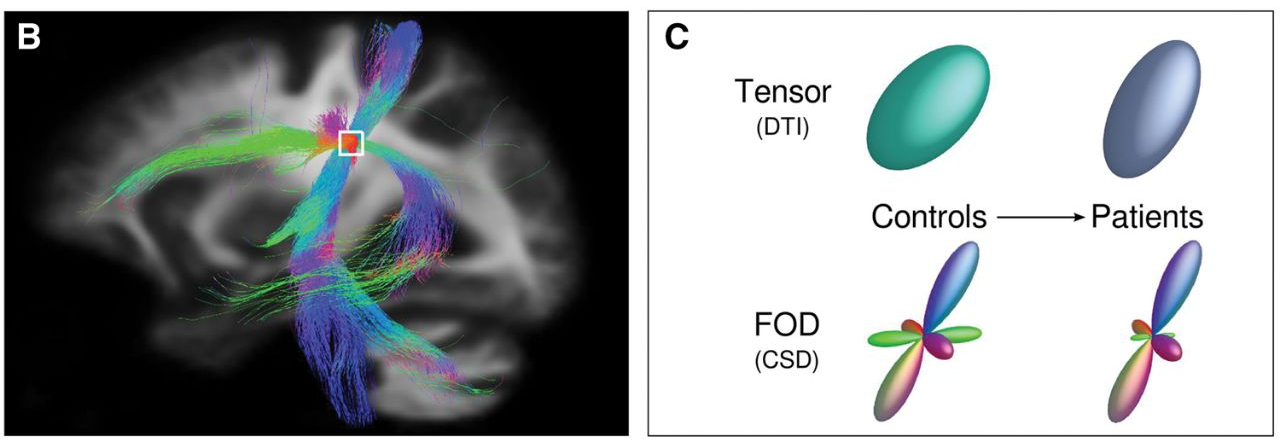
\includegraphics[width=\linewidth]{../pics/ad01_crop}
		\caption[Significant voxel-wise increases in fractional anisotropy in Alzheimer's disease compared to healthy controls]{Significant voxel-wise increases in fractional anisotropy in Alzheimer's disease compared to healthy controls; from \cite{ad}}
		\label{fig:ad01}
	\end{figure}

	\begin{figure}
		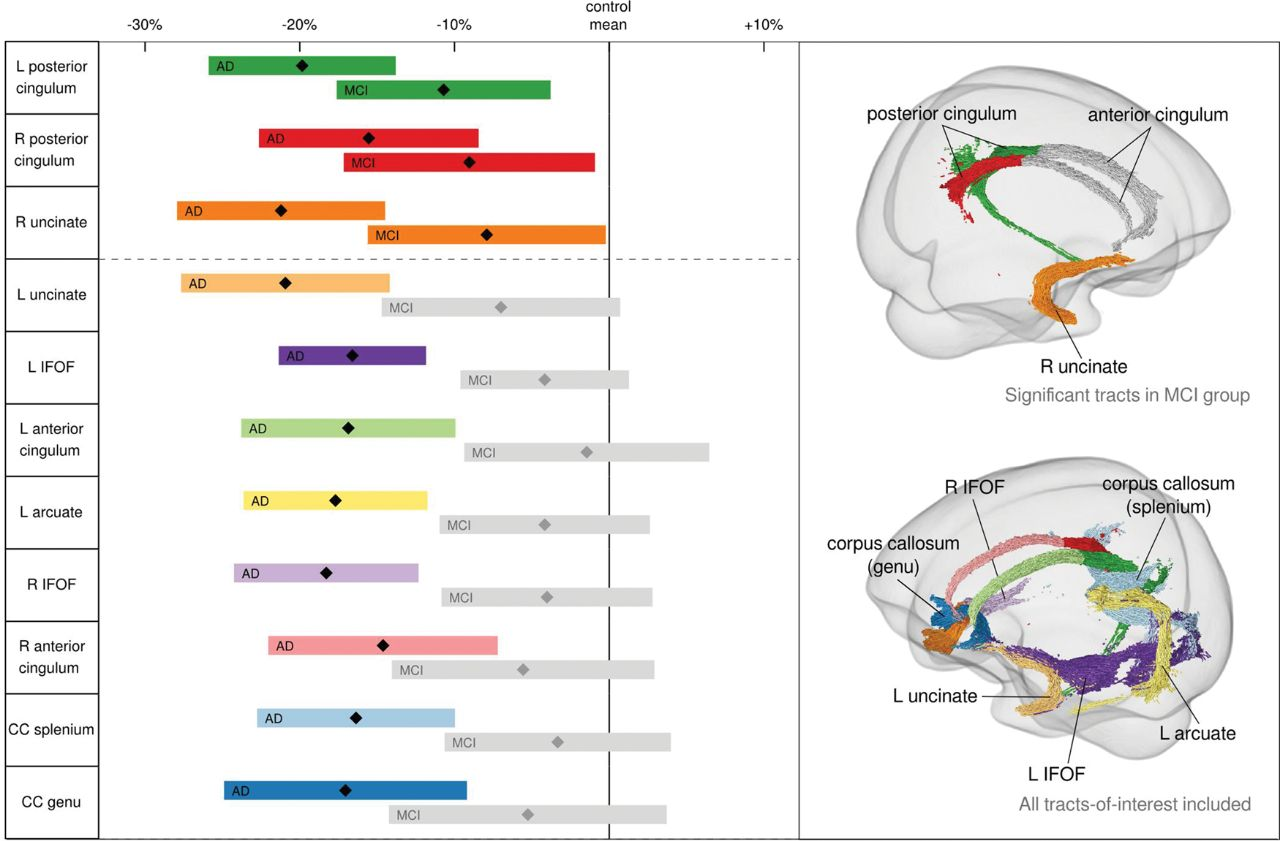
\includegraphics[width=\linewidth]{../pics/ad02}
		\caption[Significant tracts in MCI from tract-of-interest analysis comparing diagnostic groups]{Significant tracts in MCI from tract-of-interest analysis comparing diagnostic groups; from \cite{ad}}
		\label{fig:ad02}
	\end{figure}
	
	\chapter{Evaluation}
	In 2009, the \acrfull{nih}, a part of the U.S. Department of Health and Human Services\newcite{nih_about}, launched the \acrfull{hcp} in ''an ambitious effort to map the neural pathways that underlie human brain function.''\newcite{nih_connectome}. Its goal is to advance the capabilities of both imaging and analysis of human brain connections, hoping this will accelerate the progress of human connectomics. 
	
	\acrshort{hcp} is carried out by two research consortia:
	\begin{itemize}
		\item \emph{Harvard/MGH-UCAL}: Massachusetts General Hospital/Harvard University and the University of California Los Angeles (UCLA), focuses on creating a new magnetic resonance imager optimized for measuring connectome data
		\item \emph{WU/Minn}: Washington University in St. Louis/University of Minnesota/Oxford University, focuses on mapping macroscopic brain circuitry and researching its connection to behavior. That includes data acquisition from 1200 subjects with a magnetic induction of $ 3T $ and from 200 subjects at $ 7T $\newcite{wuminn}. 
	\end{itemize}
	Main directives of both consortia also include the improvement of existing and development of new imaging protocols and processing techniques. The collected data and software are made publicly available, the process of which is managed by the \Gls{CCF}. 
	
	First results published only few years after the initiation of \acrshort{hcp} inspired further projects, i.e. the \Gls{LHCP} acquiring imaging data across all ages split into four subprojects (prenatal, 0-5, 6-21, and 36-100+ years), as well as several projects focusing on connectomes related to diseases, such as \acrshort{ad}.

	\printglossary[type=gloss_terms]
	\printglossary[type=gloss_acr]
	\nocite{*}
	\bibliographystyle{unsrt}
	\bibliography{lib}
\end{document}